\documentclass[../../../topic_calculus]{subfiles}

\begin{document}

\sectionline
\section{曲面と山の形状}
%\marginnote{\refbookA}

曲面$z=x^2-y^2$の局所的な形状は、身近なところにも現れている。

\br

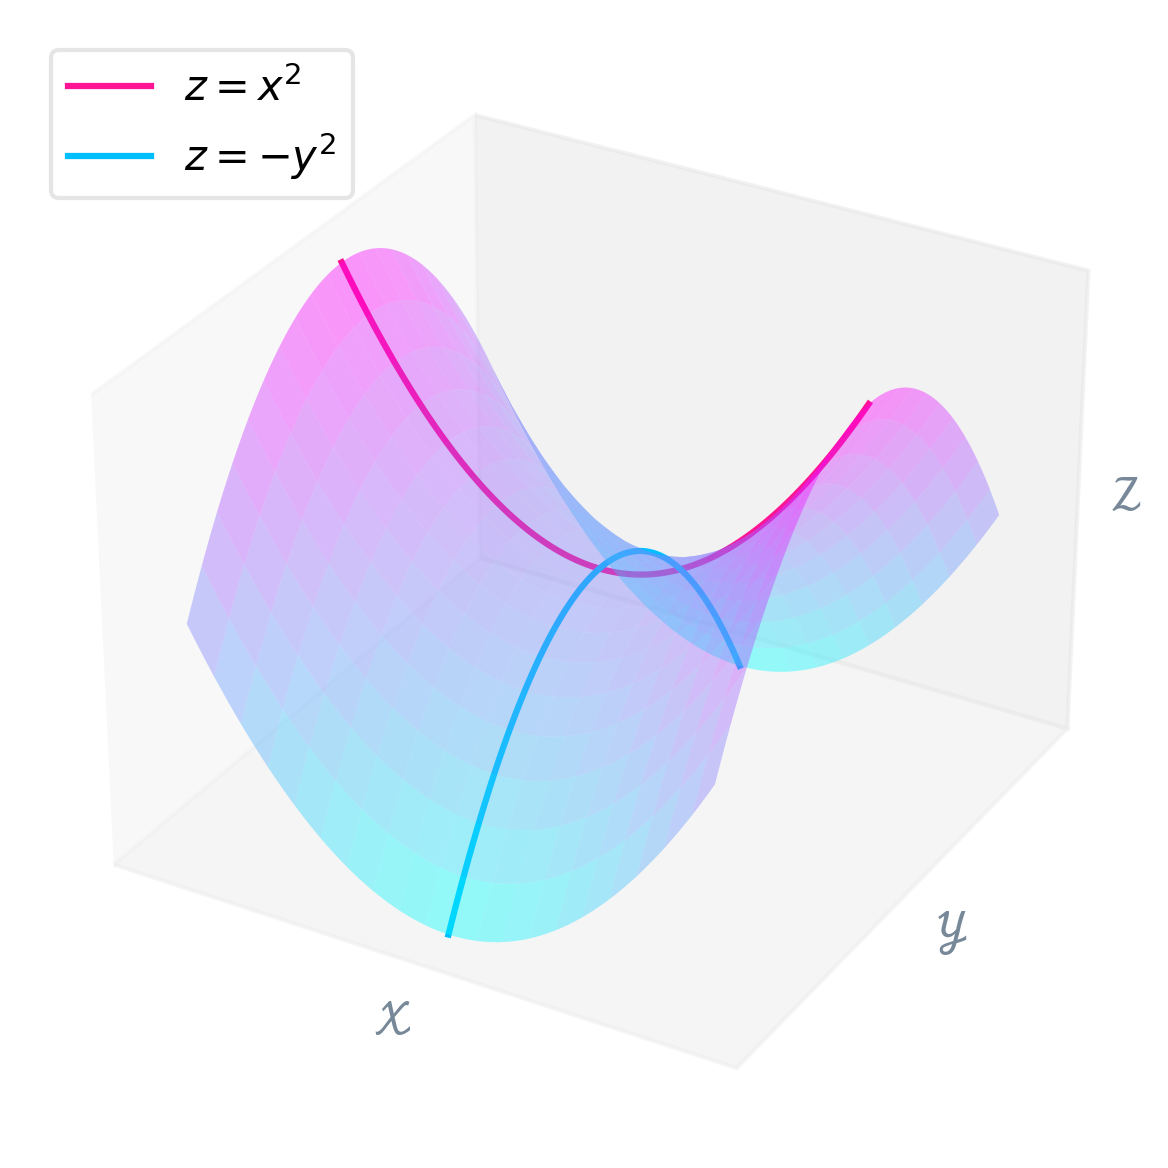
\includegraphics{../python/graph_x-pow2-sub-y-pow2_02.png}

上の図では、$y=0$としたときのグラフ$z=x^2$を赤線で、$x = 0$としたときのグラフ$z=-y^2$を青線で示した。

\br

これらのグラフは、原点$(0,0,0)$で交わっている。

この交点は、
\begin{itemize}
  \item 山の峠に見立てて\keyword{峠点}
  \item $z=x^2$の凹みを馬の背に見立てて\keyword{鞍点}(乗馬の際に鞍を置く場所)
\end{itemize}
などと呼ばれる。

\br

山が連なっているような山脈を越えて向こう側に行きたいとすると、できるだけ登りが少ない経路を選ぶだろう。

このような往来によって踏み固められてできた道が\keyword[Cerulean]{山脈越えの道}(グラフでは$x=0$の場合の放物線$z = -y^2$)である。

\br

旅人が\keyword[Cerulean]{山脈越えの道}を登っていくと、峠はその道沿いではいちばん高い地点になっている。

峠で左右を見ると、山(グラフでは$x=\text{\bfseries 定数}$の場合の放物線)が続いている。

\br

いま登ってきた山脈越えの道と垂直に交わっている\keyword[Rhodamine]{尾根道}(グラフでは$y=0$の場合の放物線$z = x^2$)があるかもしれない。

\keyword[Rhodamine]{尾根道}沿いに歩けば、峠はその前後ではいちばん低い場所になっている。

\end{document}
